\pagebreak

\section{Vehicle Ad-Hoc Networking (\ac{VANET})}
\ac{VANET} is a subclass of \ac{MANET}. The technology allows \ac{IVC} and is used for various reasons. With \ac{IVC}, vehicles are able to communicate with other vehicles within their vicinity. This is known as \ac{V2V}. Applications to \ac{V2V} communications include vehicle platooning and forward collision avoidance. In this survey \citep{Kiess2007OnCommunication}, it outlines a \ac{V2V} application of an emergency braking signal that is propagated through vehicles along the road when a vehicle suddenly stops. As vehicles behind receive this information, they may be able to react on time. Other applications include speed management to avoid traffic jams and an altered emergency response vehicle distress signal.

There are other forms of \ac{VANET} models. Those include \ac{V2I}, \ac{V2D}, and \ac{V2G}. \ac{V2I} allows vehicle communications with \ac{V2I} supported junctions, traffic lights, as well as road signs.


VANET models allow parking information shared from vehicle to vehicle within a vicinity. For example, when a car gives up a parking spot, it may announce as so, so that the information may be propagated to a vehicle nearby looking for a space.

An increasing amount of vehicles are being equipped with on-board wireless communication units in order to facilitate wireless network among vehicles and their environments \citep{Lin2008SecurityNetworks}. Thus more vehicles on the road could have the potential to support a smart parking system network environment.

In another paper \citep{Panayappan2007VANET-basedAvailability}, the proposal brought forward involves a Voronoi diagram in order to dissect the regions of an urban area.

\begin{figure}[H]
    \centering
    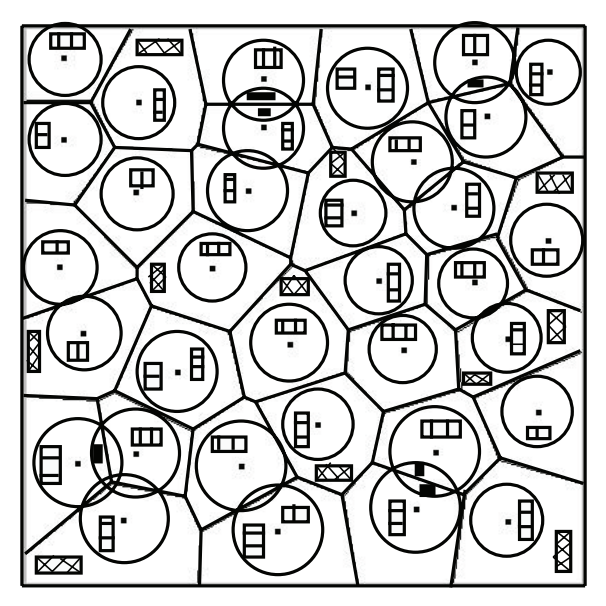
\includegraphics[width=0.5\linewidth]{./Images/VORONOI.png}
    \caption{Voronoi Model}
    \label{figure:voronoi}
\end{figure}

Shown in figure \ref{figure:voronoi} is a Voronoi model dissecting each section of an urban area. The paper proposes that a road side unit (RSU) should be placed at the center of each individual sector; to handle all the information regarding parking information within its corresponding sector. Thus, each unit handles the occupancy levels of the parking spaces available to their designated areas and the vehicles with on-board wireless communications units may be able to communicate with each sector that it traverses through.

Although, the drawbacks with this type of implementation would be the cost, as the additional RSUs need to be deployed as well as parking sensors that monitor the parking spaces. This may be necessary for a VANET based system, however unlikely within an urban setting, there may be times where a vehicle is isolated from any nearby networks thus the lack of information for it would render it impossible to receive any type of information.

Furthermore, introduction of a VANET based system would also include distributed system models which have been researched much more thoroughly in terms of computer networks.